\chapter{Overview of VAEs}\label{chap:vae}

\section{Introduction}

This chapter recalls the Variational Auto-Encoder (VAE) and introduces
the notions used for the Deep Kalman Filter in the next chapter. For a
complete treatment, see Murphy's book \cite{murphy2023probabilistic}.

A VAE has two components (Figure~\ref{fig:vae}):
\begin{itemize}
    \item an \textbf{encoder}, which maps an input
    $\textcolor{red}{\mathbf{x}}$ to a distribution over a latent variable
    $\textcolor{green!50!black}{\mathbf{z}}$;
    \item a \textbf{decoder}, which maps a latent value
    $\textcolor{green!50!black}{\mathbf{z}}$ to a distribution over the
    data space, from which a reconstruction
    $\textcolor{red}{\hat{\mathbf{x}}}$ is obtained.
\end{itemize}

\begin{figure}[ht!]
    \centering
    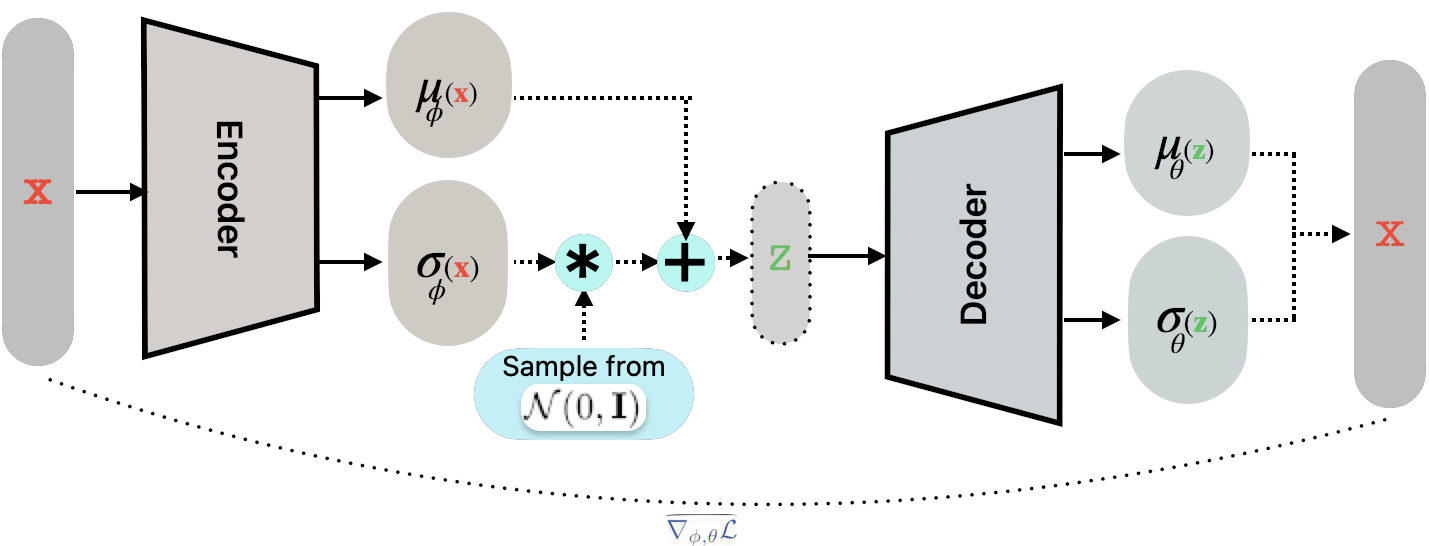
\includegraphics[width=300px]{./Images/vae.png}
    \caption{Variational Auto-Encoder}
    \label{fig:vae}
\end{figure}

\section{The model}

Let $\{\mathbf{x}^{(1)}, \dots, \mathbf{x}^{(N)}\}$ be a dataset of
independent data points. Each data point is assumed to be generated by
the following process.

\paragraph{Generative model (decoder).}
\begin{equation*}
    p(\mathbf{z}) = \mathcal{N}(\mathbf{z};\ \mathbf{0}, \mathbf{I}),
    \qquad
    p_{\theta}(\mathbf{x} \mid \mathbf{z}) =
    \mathcal{N}\big(\mathbf{x};\ \boldsymbol{\mu}_{\theta}(\mathbf{z}),\
    \mathrm{diag}(\boldsymbol{\sigma}^2_{\theta}(\mathbf{z}))\big),
\end{equation*}
where $\boldsymbol{\mu}_{\theta}$ and $\boldsymbol{\sigma}^2_{\theta}$
are computed by a neural network with parameters $\theta$.

\paragraph{Inference model (encoder).}
The posterior
$p_\theta(\mathbf{z} \mid \mathbf{x}) =
p_\theta(\mathbf{x} \mid \mathbf{z})\,p(\mathbf{z})/p_\theta(\mathbf{x})$
is intractable, because
$p_\theta(\mathbf{x}) = \int p_\theta(\mathbf{x} \mid \mathbf{z})\,
p(\mathbf{z})\,d\mathbf{z}$ has no closed form when the decoder is a
neural network. It is approximated by
\begin{equation*}
    q_{\phi}(\mathbf{z} \mid \mathbf{x}) =
    \mathcal{N}\big(\mathbf{z};\ \boldsymbol{\mu}_{\phi}(\mathbf{x}),\
    \mathrm{diag}(\boldsymbol{\sigma}^2_{\phi}(\mathbf{x}))\big),
\end{equation*}
where $\boldsymbol{\mu}_{\phi}$ and $\boldsymbol{\sigma}^2_{\phi}$ are
computed by a second neural network with parameters $\phi$. A single
network serves every data point; this is called \emph{amortised}
inference.

\section{The Evidence Lower Bound}

\subsection{Why it is a lower bound}

For any distribution $q(\mathbf{z} \mid \mathbf{x})$ whose support
contains that of the posterior,
\begin{align*}
    \log p_\theta(\mathbf{x})
    &= \log \int q(\mathbf{z} \mid \mathbf{x})\,
       \frac{p_\theta(\mathbf{x}, \mathbf{z})}{q(\mathbf{z} \mid
       \mathbf{x})}\,d\mathbf{z}
     = \log \E_{q(\mathbf{z} \mid \mathbf{x})}\!\left[
       \frac{p_\theta(\mathbf{x}, \mathbf{z})}{q(\mathbf{z} \mid
       \mathbf{x})}\right] \\
    &\geq \E_{q(\mathbf{z} \mid \mathbf{x})}\!\left[\log
       \frac{p_\theta(\mathbf{x}, \mathbf{z})}{q(\mathbf{z} \mid
       \mathbf{x})}\right] \;=:\; \mathcal{L}(\theta, \phi; \mathbf{x}),
\end{align*}
by Jensen's inequality, since $\log$ is concave. This is the
\textbf{Evidence Lower Bound} (ELBO). The size of the gap is known
exactly. Writing
$p_\theta(\mathbf{x}, \mathbf{z}) = p_\theta(\mathbf{x})\,
p_\theta(\mathbf{z} \mid \mathbf{x})$ inside the logarithm gives
\begin{equation}
    \log p_\theta(\mathbf{x}) = \mathcal{L}(\theta, \phi; \mathbf{x}) +
    \KL\big(q_\phi(\mathbf{z} \mid \mathbf{x}) \,\|\,
    p_\theta(\mathbf{z} \mid \mathbf{x})\big).
    \label{eq:elbo_gap}
\end{equation}

\begin{inwords}
The ELBO is below the log-likelihood by exactly the KL divergence
between the encoder and the true posterior. Maximising the ELBO over
$\phi$ therefore makes the encoder a better approximation of the
posterior. Maximising it over $\theta$ pushes the log-likelihood up.
The bound is tight when the encoder equals the posterior.
\end{inwords}

\subsection{Reconstruction and regularisation terms}

Writing $p_\theta(\mathbf{x}, \mathbf{z}) =
p_\theta(\mathbf{x} \mid \mathbf{z})\,p(\mathbf{z})$ instead gives the
usual form
\begin{equation*}
    \mathcal{L}(\theta, \phi; \mathbf{x}) =
    \underbrace{\E_{q_{\phi}(\mathbf{z} \mid \mathbf{x})}
    \big[\log p_{\theta}(\mathbf{x} \mid \mathbf{z})\big]}_{
    \text{reconstruction term}}
    \;-\;
    \underbrace{\KL\big(q_{\phi}(\mathbf{z} \mid \mathbf{x}) \,\|\,
    p(\mathbf{z})\big)}_{\text{regularisation term}}.
\end{equation*}
\begin{itemize}
    \item The \textbf{reconstruction term} rewards latent codes from
    which the decoder assigns high likelihood to the input. Its negative
    is the reconstruction loss.
    \item The \textbf{regularisation term} penalises encoders that move
    away from the prior. With Gaussian $q_\phi$ and prior it has a closed
    form (Appendix~\ref{sec:elbo_regularization}).
\end{itemize}

\section{Training the VAE}

The VAE is trained by minimising $-\mathcal{L}$, averaged over the
dataset, with stochastic gradient descent or one of its variants. The
expectation in the reconstruction term is estimated with one (or a few)
samples $\mathbf{z} \sim q_\phi(\mathbf{z} \mid \mathbf{x})$. Since a
Monte Carlo average of samples from $q_\phi$ is an unbiased estimate of
the expectation, the gradient of the estimate is an unbiased estimate of
the gradient, provided the sample can be differentiated with respect to
$\phi$.

\subsection{Reparameterisation trick}

That is what the reparameterisation trick provides. Instead of sampling
$\mathbf{z}$ from $q_\phi$ directly, write
\begin{equation*}
    \mathbf{z} = \boldsymbol{\mu}_{\phi}(\mathbf{x}) +
    \boldsymbol{\sigma}_{\phi}(\mathbf{x}) \odot \boldsymbol{\epsilon},
    \qquad \boldsymbol{\epsilon} \sim \mathcal{N}(\mathbf{0},
    \mathbf{I}),
\end{equation*}
where $\boldsymbol{\sigma}_{\phi}$ is the vector of standard deviations
(the square root of the variances) and $\odot$ the element-wise product.
The randomness is now in $\boldsymbol{\epsilon}$, which does not depend
on $\phi$, so $\mathbf{z}$ is a differentiable function of $\phi$ for
fixed $\boldsymbol{\epsilon}$.

\section{Summary}

A VAE approximates the intractable posterior
$p_\theta(\mathbf{z} \mid \mathbf{x})$ by an encoder
$q_\phi(\mathbf{z} \mid \mathbf{x})$ and trains encoder and decoder
together by maximising
\begin{equation*}
    \mathcal{L}(\theta, \phi; \mathbf{x}) =
    \E_{q_\phi(\mathbf{z} \mid \mathbf{x})}[\log
    p_\theta(\mathbf{x} \mid \mathbf{z})]
    - \KL(q_\phi(\mathbf{z} \mid \mathbf{x}) \,\|\, p(\mathbf{z}))
    = \log p_\theta(\mathbf{x}) -
    \KL(q_\phi(\mathbf{z} \mid \mathbf{x}) \,\|\,
    p_\theta(\mathbf{z} \mid \mathbf{x})).
\end{equation*}
The Deep Kalman Filter applies the same recipe to a whole sequence, with
a latent variable per time step linked by a Markov chain.
